\subsection{Упражнение 1}

Создайте треугольный сигнал и напечатайте его. Примените diff к сигналу и напечатайте результат. Вычислите спектр треугольного сигнала, примените differentiate и напечатайте результат. Преобразуйте спектр обратно в сигнал и напечатайте его. Есть ли различия в воздействии diff и differentiate на этот сигнал?

\begin{lstlisting}[language=Python]
wave = TriangleSignal(freq=440).make_wave(duration=0.01, framerate=44100)
wave.plot()
decorate(xlabel='Time (s)')
\end{lstlisting}
\begin{figure}[H]
	\begin{center}
		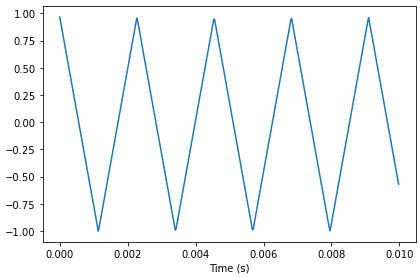
\includegraphics[scale=1]{fig/lab09/lab9_1.png}
		\caption{График сигнала}
	\end{center}
\end{figure}

\begin{lstlisting}[language=Python]
diff_wave = wave.diff()
diff_wave.plot()
decorate(xlabel='Time (s)')
\end{lstlisting}
\begin{figure}[H]
	\begin{center}
		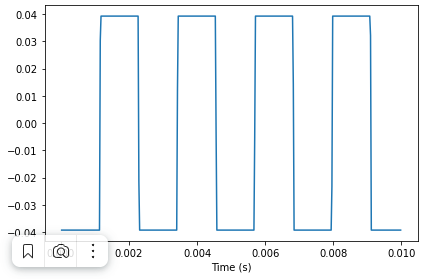
\includegraphics[scale=1]{fig/lab09/lab9_2.png}
		\caption{Сигнал после применения diff}
	\end{center}
\end{figure}

В итоге получили прямоугольный сигнал с такой же частотой.

\begin{lstlisting}[language=Python]
differentiate_wave = wave.make_spectrum().differentiate().make_wave()
differentiate_wave.plot()
decorate(xlabel='Time (s)')
\end{lstlisting}
\begin{figure}[H]
	\begin{center}
		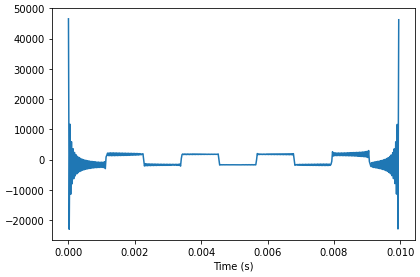
\includegraphics[scale=1]{fig/lab09/lab9_3.png}
		\caption{Сигнал после применения differentiate}
	\end{center}
\end{figure}

Из графика видно, что начало и конец интервала сильно зашумлены. Возможно, это связано с невозможностью определения произодной.

\subsection{Упражнение 2}

Создайте прямоугольный сигнал и напечатайте его. Примените cumsum и напечатайте результат. Вычислите спектр прямогоульного сигнала, примените integrate и напечатайте результат. Преобразуйте спектр обратно в сигнал и напечайте его. Есть различия в воздействии cumsum и integrate на этот сигнал?

\begin{lstlisting}[language=Python]
wave = SquareSignal(freq=100).make_wave(duration=0.1, framerate=44100)
wave.plot()
decorate(xlabel='Time (s)')
\end{lstlisting}
\begin{figure}[H]
	\begin{center}
		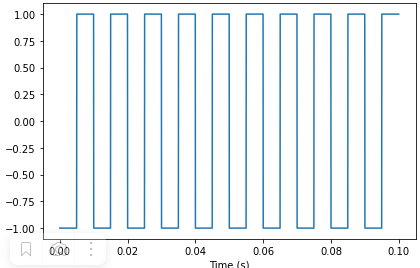
\includegraphics[scale=1]{fig/lab09/lab9_4.png}
		\caption{Рассматриваемый сигнал}
	\end{center}
\end{figure}

Кумулятивная сумма:

\begin{lstlisting}[language=Python]
cumsum_wave = wave.cumsum()
cumsum_wave.plot()
decorate(xlabel='Time (s)')
\end{lstlisting}
\begin{figure}[H]
	\begin{center}
		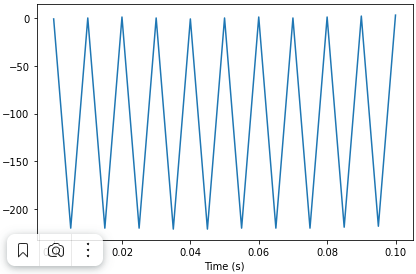
\includegraphics[scale=1]{fig/lab09/lab9_5.png}
		\caption{Рассматриваемый сигнал после применения cumsum}
	\end{center}
\end{figure}

Получили треугольный сигнал.

Теперь интеграл спектра:

\begin{lstlisting}[language=Python]
int_spec = wave.make_spectrum().integrate()
int_spec.hs[0] = 0
int_wave = int_spec.make_wave()
int_wave.plot()
decorate(xlabel='Time (s)')
\end{lstlisting}
\begin{figure}[H]
	\begin{center}
		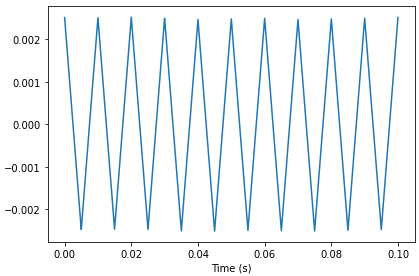
\includegraphics[scale=1]{fig/lab09/lab9_6.png}
		\caption{Рассматриваемый сигнал после применения integrate}
	\end{center}
\end{figure}

Воспользуемся кодом автора и "сложим" два графика с изменением масштаба.

\begin{lstlisting}[language=Python]
cumsum_wave.unbias()
cumsum_wave.normalize()
int_wave.normalize()
cumsum_wave.plot()
int_wave.plot()
\end{lstlisting}
\begin{figure}[H]
	\begin{center}
		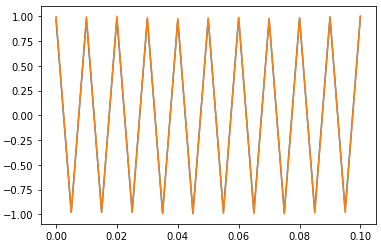
\includegraphics[scale=1]{fig/lab09/lab9_7.png}
		\caption{Сравнение полученных графиков}
	\end{center}
\end{figure}

Видим, что графики практически идентичны. Следовательно разные у них лишь амплитуды.

\subsection{Упражнение 3}

Создайте пилообразный сигнал, вычислите его спектр, а затем дважды примените integrate. Напечатйте результирующий сигнал и его спектр. Какова математическая форма сигнала? Почему он напоминает синусойду?

\begin{lstlisting}[language=Python]
wave = SawtoothSignal(freq=100).make_wave(duration=0.1, framerate=44100)
wave.plot()
decorate(xlabel='Time (s)')
\end{lstlisting}
\begin{figure}[H]
	\begin{center}
		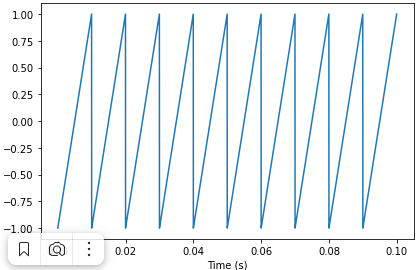
\includegraphics[scale=1]{fig/lab09/lab9_8.png}
		\caption{Пилообразный сигнал}
	\end{center}
\end{figure}

\begin{lstlisting}[language=Python]
spectrum = wave.make_spectrum().integrate().integrate()
spectrum.hs[0] = 0

wave1 = spectrum.make_wave()
wave1.plot()
decorate(xlabel='Time (s)')
\end{lstlisting}
\begin{figure}[H]
	\begin{center}
		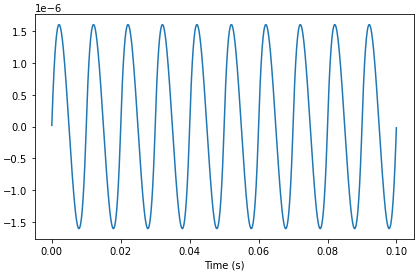
\includegraphics[scale=1]{fig/lab09/lab9_9.png}
		\caption{Изменённый сигнал}
	\end{center}
\end{figure}

Из графика видно, что сигнал действительно напоминает синусоиду. Причиной этому является фильтрация низких чистот, за исключением основной.

\begin{lstlisting}[language=Python]
wave.make_spectrum().plot(high=1000)
\end{lstlisting}
\begin{figure}[H]
	\begin{center}
		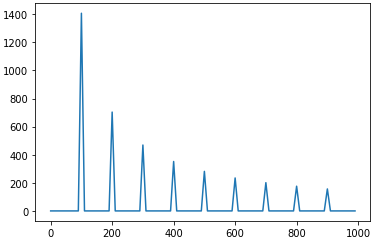
\includegraphics[scale=1]{fig/lab09/lab9_10.png}
		\caption{Спектр исходного сигнала}
	\end{center}
\end{figure}

\begin{lstlisting}[language=Python]
wave1.make_spectrum().plot(high=1000)
\end{lstlisting}
\begin{figure}[H]
	\begin{center}
		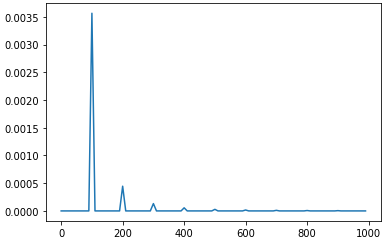
\includegraphics[scale=1]{fig/lab09/lab9_11.png}
		\caption{Спектр нового сигнала}
	\end{center}
\end{figure}


\subsection{Упражнение 4}

Создайте CubicSignal, определённый в thinkdsp. Вычислите вторую разность, дважды применив diff. Как выглядит результат? Вычислите вторую разность, дважды применив differentiate к спектру. Похожи ли результаты? Распечатйте фильтры, соответсвующие второй разнице и второй производной. Сравните их.

Тут надо точно подобрать параметры, чтобы сигнал красиво отображался при таком маленьком frametime.

\begin{lstlisting}[language=Python]
wave = CubicSignal(freq=0.01).make_wave(duration=1000, framerate=1)
wave.plot()
\end{lstlisting}
\begin{figure}[H]
	\begin{center}
		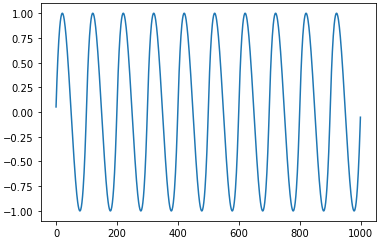
\includegraphics[scale=1]{fig/lab09/lab9_12.png}
		\caption{Кубический сигнал}
	\end{center}
\end{figure}

Первая разность - параболы.

\begin{lstlisting}[language=Python]
d1_wave = wave.diff()
d1_wave.plot()
\end{lstlisting}
\begin{figure}[H]
	\begin{center}
		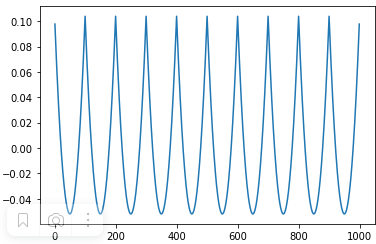
\includegraphics[scale=1]{fig/lab09/lab9_13.png}
		\caption{Первая разность}
	\end{center}
\end{figure}

Вторая разность - пилообразный сигнал.

\begin{lstlisting}[language=Python]
d2_wave = d1_wave.diff()
d2_wave.plot()
\end{lstlisting}
\begin{figure}[H]
	\begin{center}
		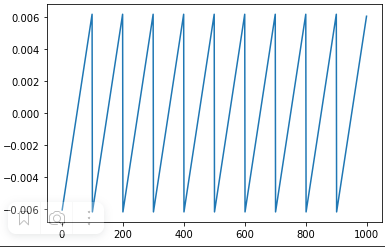
\includegraphics[scale=1]{fig/lab09/lab9_14.png}
		\caption{Вторая разность}
	\end{center}
\end{figure}

При двойном дифференцировании получаем звон в пилообразном сигнале, звон связан со сложностями в вычислении производной, как и ранее.

\begin{lstlisting}[language=Python]
spectrum = wave.make_spectrum().differentiate().differentiate()
di_wave = spectrum.make_wave()
di_wave.plot()
decorate(xlabel='Time (s)')
\end{lstlisting}
\begin{figure}[H]
	\begin{center}
		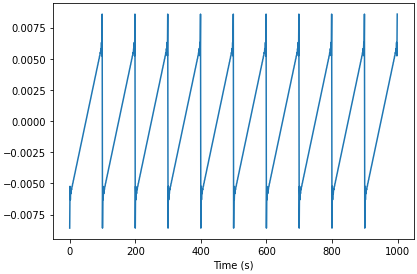
\includegraphics[scale=1]{fig/lab09/lab9_15.png}
		\caption{Полученный сигнал со звоном}
	\end{center}
\end{figure}

Фильтры:
\begin{lstlisting}[language=Python]
diff_filter.plot(label='2nd diff')
deriv_filter.plot(label='2nd deriv')

decorate(xlabel='Frequency (Hz)',
                 ylabel='Amplitude ratio')
\end{lstlisting}

\begin{figure}[H]
	\begin{center}
		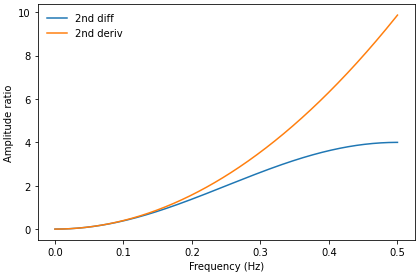
\includegraphics[scale=1]{fig/lab09/lab9_16.png}
		\caption{Полученные фильтры}
	\end{center}
\end{figure}

Мы получили фильтры для усиления высокочастотных компонент. Производная является пароболой, поэтому она усиливает сильней. Разность хорошо аппроксимирует только на низких частотах, а далее получаем существенное отклонение.

\subsection{Вывод}

В ходе данной ЛР были рассмотрены соотношения между окнами во временной области и фильтрами в частотной. Также были рассмотрены конечные разности, аппроксимирующее дифференцирование и накапливающие суммы с аппроксимирующим интегрированием.